\documentclass[french,bookmarks]{beamer}

\usepackage{tikz}
\usetikzlibrary{angles, quotes, graphdrawing.trees, tikzmark, decorations.markings,decorations.pathreplacing, positioning, 3d, shapes.misc, shapes.geometric, automata, arrows,calc,positioning}
\usetheme{default}
\usecolortheme{seahorse}

\usepackage{lmodern}
\usepackage{babel}
\usepackage[T1]{fontenc}
\usepackage{stmaryrd}

\usepackage{xparse}
\usepackage[most,breakable,listings]{tcolorbox}

\usefonttheme[onlymath]{serif}

%\newfontfamily{\EBGaramond}{EBGaramond}[RawFeature={+clig,+liga,+cv11,+cv90,+calt,+ccmp,+swsh},Ligatures=TeX]

%\defaultfontfeatures{RawFeature={+hlig,+clig,+liga,+cv11,+cv90,+calt,+ccmp,+swsh},Ligatures=TeX} %+dlig ?


\definecolor{main1} {RGB}{8, 127, 196}

\definecolor{main1comp} {RGB}{218, 65, 103}
\definecolor{main1comp2} {RGB}{119, 186, 153}
\definecolor{main1white} {RGB}{121, 129, 134}
\definecolor{main1white2} {RGB}{204, 204, 204}
\definecolor{main2} {RGB}{64, 115, 192}
\definecolor{main3} {RGB}{96, 102, 183}
\definecolor{main4} {RGB}{120, 86, 169}
\definecolor{main5} {RGB}{139, 69, 149}
\definecolor{main6} {RGB}{152, 51, 126}
\definecolor{main7} {RGB}{158, 30, 100}
\definecolor{main8} {RGB}{159, 4, 72}
\definecolor{main9} {RGB}{153, 0, 44}
\definecolor{main10} {RGB}{142, 1, 15}
\definecolor{main10comp} {RGB}{250, 126, 97}
\definecolor{main10comp2} {RGB}{63, 136, 197}

\definecolor{main20} {RGB}{7, 163, 106}
\definecolor{main21} {RGB}{184, 0, 0}

\definecolor{ocamlColor} {RGB}{242, 130, 17}

\setbeamercolor{titlelike}{parent=structure,bg=main3,fg=white}

\DeclareDocumentCommand\declarecours{mmmm}{
    \newtcbtheorem[]{AUX_#1}{\vphantom{Ép}#2}{
        breakable,
        enhanced,
        top = 5mm,
        before skip balanced = \tcboxedtitleheight/3,
        separator sign={\quad},
        %separator sign={\ \ding{228}},
        %if odd page={
            attach boxed title to top left={
                yshift=-\tcboxedtitleheight/2,
                xshift=-2mm
            },
            boxed title style={
                frame code={
                    \path[fill = #4!90]
                    %left color=#4!90!gray!90, right color=#4!85!gray!75] 
                        (frame.north west) -- 
                        (frame.north east) -- 
                        (frame.south east) -- 
                        (frame.south west) -- 
                        cycle;
                },
                interior engine=empty,
            },
        %}{
        %    attach boxed title to top right={
        %        yshift=-\tcboxedtitleheight/3,
        %        xshift=2mm
        %    },
        %    boxed title style={
        %        frame code={
        %            \path[right color=#4!90!gray!90, left color=#4!85!gray!75]
        %                (frame.north west) -- 
        %                (frame.north east) -- 
        %                (frame.south east) -- 
        %                (frame.south west) -- 
        %                cycle;
        %        },
        %        interior engine=empty,
        %    }
        %},
        fonttitle           = \sffamily,
        %borderline west     = {.5pt}{0pt}{#4!85!gray!50},
        %borderline north    = {\tcboxedtitleheight/3}{-\tcboxedtitleheight/3}{#4!85!gray!50},
        %borderline east     = {.5pt}{0pt}{#4!85!gray!50},
        %borderline south    = {.5pt}{0pt}{#4!85!gray!50},
        interior style      = {
            fill            = #4!10
            %left color      = #4!100!gray!8,
            %middle color    = #4!75!gray!7,
            %right color     = #4!50!gray!6
        },
        sharp corners   = downhill,
        arc             = 0 cm,
        boxrule         = 0pt,
        frame hidden%,
        %drop fuzzy shadow=#4!3
    }{#3}
    \newenvironment{#1}[2]{
        \begingroup
        \renewcommand{\bf}[1]{{\color{#4}\textbf{####1}}}
        \newcommand{\hg}[1]{\begingroup\color{#4}{####1}\endgroup}
        \newcommand{\hgu}[1]{\begingroup\color{#4}\underline{####1}\endgroup}
        \newcommand{\hguo}[1]{\begingroup\colorlet{cb@savedHGUO}{.}\color{#4}\underline{\color{cb@savedHGUO}####1}\endgroup}
        \newcommand{\boxedcol}[1]{\begingroup\colorlet{cb@savedBOX}{.}\color{#4}\boxed{\color{cb@savedBOX}####1}\endgroup}
        \begin{AUX_#1*}{##1}{##2}
    }{
        \end{AUX_#1*}
        \endgroup
        \global\def\nproofcolor{#4}
    }
    \expandafter\NewDocumentCommand\csname #3ref\endcsname{m}{\textsc{\smartref{#3:##1} }}
}

\declarecours{bdefinition}{Définition}{def}{main1}
\declarecours{bproperty}{Propriété}{prop}{main3}
\declarecours{blemma}{Lemme}{lem}{main6}
\declarecours{btheorem}{Théorème}{th}{main10}
\declarecours{bcorrolary}{Corollaire}{cor}{main9}

\DeclareDocumentCommand\declarecoursalt{mmmm}{
    \newtcbtheorem[]{AUX_#1}{#2}{
        theorem name,
        breakable,
        enhanced,
        top = 3mm,
        separator sign={\quad},
        attach boxed title to top center={
            yshift=-\tcboxedtitleheight/2,
        },
        colframe            = {#4},
        borderline west     = {.5pt}{0pt}{#4},
        borderline north    = {.5pt}{0pt}{#4},
        borderline east     = {.5pt}{0pt}{#4},
        borderline south    = {.5pt}{0pt}{#4},
        colback             = #4!1,
        fonttitle           = \sffamily,
        sharp corners       = downhill,
        arc                 = 0 cm,
        boxrule             = 0pt,
        frame hidden,
        %drop fuzzy shadow=#4!10!white,
        boxed title style={
        frame code={
            \path[left color=#4!95!gray!90,right color=#4!95!gray!90, middle color=#4!70!gray!90, fill=white] 
                    ([xshift=-2mm]frame.north west) -- 
                    ([xshift=2mm]frame.north east) -- 
                    ([xshift=2mm]frame.south east) -- 
                    ([xshift=-2mm]frame.south west) -- 
                    cycle;
        },
        interior engine=empty,
        }
    }{#3}
    \newenvironment{#1}[2]{
        \begingroup
        \renewcommand{\bf}[1]{{\color{#4}\textbf{####1}}}
        \newcommand{\hg}[1]{\begingroup\color{#4}{####1}\endgroup}
        \newcommand{\hgu}[1]{\begingroup\color{#4}\underline{####1}\endgroup}
        \newcommand{\hguo}[1]{\begingroup\colorlet{cb@savedHGUO}{.}\color{#4}\underline{\color{cb@savedHGUO}####1}\endgroup}
        \newcommand{\boxedcol}[1]{\begingroup\colorlet{cb@savedBOX}{.}\color{#4}\boxed{\color{cb@savedBOX}####1}\endgroup}
        \begin{AUX_#1*}{##1}{##2}
    }{
        \end{AUX_#1*}
        \endgroup
    }
    \expandafter\NewDocumentCommand\csname #3ref\endcsname{m}{\textsc{\smartref{#3:##1}}}
}

\declarecoursalt{bexample}{Exemple}{example}{main2}
\declarecoursalt{bexercise}{Exercice}{exo}{main20}
\declarecours{bexotd}{Exercice}{exotd}{main20}
\declarecoursalt{bwarning}{Avertissement}{warn}{main21}

\declarecoursalt{bform}{}{form}{black}


\newenvironment{psse}{
    \begin{enumerate}[label=\textrm{\rmfamily\itshape(\roman*)}]
}{
    \end{enumerate}
}

\newcommand{\pssenum}[1]{\textrm{\rmfamily\itshape(#1)}}

\newenvironment{expcom}{
    \begingroup
    \begin{tcolorbox}[
        breakable,
        enhanced,
        interior style      = {
            left color      = main1white2!65!gray!8,
            middle color    = main1white2!50!gray!7,
            right color     = main1white2!35!gray!6
        },
        %borderline north    = {.3pt}{0pt}{main1white!10},
        %borderline south    = {.3pt}{0pt}{main1white!10},
        %borderline west     = {2pt}{0pt}{colexp!85!gray!50},
        sharp corners       = downhill,
        frame hidden,
        arc                 = 0 cm,
        boxrule             = 0 cm,
        nobeforeSTYLE,
        noafterSTYLE,
        overlay={\begin{tcbclipinterior}
            \path[top color=colexp!85!gray!45, middle color=colexp!85!gray!55, bottom color=colexp!85!gray!55, fill=white] 
                    (interior.north west) -- 
                    ([xshift=2pt]interior.north west) -- 
                    ([xshift=2pt]interior.south west) -- 
                    (interior.south west) -- 
                    cycle;
                    
        \end{tcbclipinterior}}
    ]
        \begin{proofpure}[Compte-rendu]
}{
        \end{proofpure}
    \end{tcolorbox}
    \endgroup
}

\newenvironment{notation}{
    \begingroup
    \begin{tcolorbox}[
        breakable,
        enhanced,
        interior style      = {
            left color      = main1white2!65!gray!8,
            middle color    = main1white2!50!gray!7,
            right color     = main1white2!35!gray!6
        },
        sharp corners       = downhill,
        frame hidden,
        arc                 = 0 cm,
        boxrule             = 0 cm,
        nobeforeSTYLE,
        noafterSTYLE,
        overlay={\begin{tcbclipinterior}
            \path[top color=main1!95!gray!90, bottom color=main1!90!gray!70, fill=white] 
                    (interior.north west) -- 
                    ([xshift=2pt]interior.north west) -- 
                    ([xshift=2pt]interior.south west) -- 
                    (interior.south west) -- 
                    cycle;
                    
        \end{tcbclipinterior}}
    ]
        \small\textbf{\color{main1!95!gray!90} \textsf{(Notation)}}\newcommand{\hg}[1]{\begingroup\color{main1!95!gray!90}{##1}\endgroup}
}{
    \end{tcolorbox}
    \endgroup
}

\newenvironment{hpnote}{
    \begingroup
    \begin{tcolorbox}[
        breakable,
        enhanced,
        interior style      = {
            left color      = main1white2!65!gray!8,
            middle color    = main1white2!50!gray!7,
            right color     = main1white2!35!gray!6
        },
        sharp corners       = downhill,
        frame hidden,
        arc                 = 0 cm,
        boxrule             = 0 cm,
        nobeforeSTYLE,
        noafterSTYLE,
        overlay={\begin{tcbclipinterior}
            \path[top color=main1!85!gray!70, bottom color=main1!85!gray!50, fill=white] 
                    (interior.north west) -- 
                    ([xshift=2pt]interior.north west) -- 
                    ([xshift=2pt]interior.south west) -- 
                    (interior.south west) -- 
                    cycle;
                    
        \end{tcbclipinterior}}
    ]
        \textbf{\color{main1!95!gray!90} \textsf{(HP)}}
}{
        
    \end{tcolorbox}
    \endgroup
}
    
\newcommand{\demo}[1]{
    \begin{tcolorbox}[
        breakable,
        enhanced,
        interior style      = {
            left color      = main3!66!gray!13,
            middle color    = main3!33!gray!9,
            right color     = main3!0!gray!5
        },
        borderline north    = {.3pt}{0pt}{main3!5},
        borderline south    = {.3pt}{0pt}{main3!5},
        borderline west     = {1.5pt}{0pt}{main3!30},
        sharp corners       = downhill,
        arc                 = 0 cm,
        boxrule             = 0 cm,
    ]

        \begin{proof}
            #1
        \end{proof}
    \end{tcolorbox}
}

\newcommand{\demoth}[1]{
    \begin{tcolorbox}[
        breakable,
        enhanced,
        interior style      = {
            left color      = main10!66!gray!13,
            middle color    = main10!33!gray!9,
            right color     = main10!0!gray!5
        },
        borderline north    = {.3pt}{0pt}{main10!5},
        borderline south    = {.3pt}{0pt}{main10!5},
        borderline west     = {1.5pt}{0pt}{main10!30},
        sharp corners       = downhill,
        arc                 = 0 cm,
        boxrule             = 0 cm
    ]

        \begin{proof}
            #1
        \end{proof}
    \end{tcolorbox}
}

\newcommand{\demolm}[1]{
    \begin{tcolorbox}[
        breakable,
        enhanced,
        interior style      = {
            left color      = main6!66!gray!13,
            middle color    = main6!33!gray!9,
            right color     = main6!0!gray!5
        },
        borderline north    = {.3pt}{0pt}{main6!5},
        borderline south    = {.3pt}{0pt}{main6!5},
        borderline west     = {1.5pt}{0pt}{main6!30},
        sharp corners       = downhill,
        arc                 = 0 cm,
        boxrule             = 0 cm
    ]

        \begin{proof}
            #1
        \end{proof}
    \end{tcolorbox}
}
    
\makeatletter
\newcommand{\exlower}{%
  \begin{tikzpicture}
  \path[use as bounding box] (0,0) -- (\linewidth,0);
  \draw[color=main2, dash dot]
        (0-\kvtcb@leftlower-\kvtcb@boxsep,0) --
        (\linewidth+\kvtcb@rightlower+\kvtcb@boxsep,0);
  \end{tikzpicture}%
  }
\makeatother

\DeclareDocumentCommand\suite{m}{{\left(#1\right)_{n \in \bdN}}} 
\DeclareDocumentCommand\suiteZ{m}{{\left(#1\right)_{n \in \bdN^*}}}

\DeclareDocumentCommand\serie{}{\textstyle{\sum\limits_{n \in \bdN}}}
\newcommand{\bdRp}{\mathbb{R}_+^*}
%note : bien mettre avant ExplSyntaxOn

\DeclareDocumentCommand\guill{m}{\og #1\fg{}}

\makeatletter
\newcommand{\kmath}[1][0.65]{%
  \mathpalette\@kmath{#1}%
}
\newcommand*{\@kmath}[2]{%
  \scalebox{#2}[#2]{$#1\mathbf{\itshape k}\m@th$}%
}
\makeatother


\ExplSyntaxOn

\DeclareDocumentCommand\funlv{mg}{
  \qopname\relax o{#1}
  \IfNoValueTF{#2}{}{\p{#2}}
}

\DeclareDocumentCommand\floor{m}{\left\lfloor#1\right\rfloor}


\DeclareDocumentCommand\funlvi{m}{
    \expandafter\DeclareDocumentCommand\expandafter{\csname #1\endcsname}{g}{\funlv{#1}{##1}}
}


\DeclareDocumentCommand\funlfv{mg}{
    \mathfrak{#1}
    \IfNoValueTF{#2}{}{\left(#2\right)}
}



\DeclareDocumentCommand\asymp{g}{%
    \IfNoValueTF{#1}{\sim}{\underset{#1}{\sim}}
}

\DeclareDocumentCommand\eq{g}{
    \IfNoValueTF{#1}{=}{\underset{#1}{=}}
}

%TODO: OPTIMISER EN CAS DUN SEUL ARG
\DeclareDocumentCommand\o{gg}{
    \IfNoValueTF{#1}{\bco}{\underset{#1}{\bco}}
    \IfNoValueTF{#2}{}{\p{#2}}
}

\DeclareDocumentCommand\O{gg}{
    \IfNoValueTF{#1}{\bcO}{\underset{#1}{\bcO}}
    \IfNoValueTF{#2}{}{\p{#2}}
}

\DeclareDocumentCommand\lima{g}{
    \IfNoValueTF{#1}{\xrightarrow[]{}}{\xrightarrow[#1]{}}
}

\DeclareDocumentCommand\rleq{}{\preccurlyeq}

\newcommand{\transp}{^{\!\mathsf{T}}}
\DeclareDocumentCommand\mtrans{m}{\,{}^\mathsf{t}\!#1}
\newcommand{\ii}{\mathrm{i\mkern1mu}}
\newcommand{\jj}{\mathrm{j\mkern1mu}}

\DeclareDocumentCommand\phyavg{m}{\left\langle#1\right\rangle}

\DeclareDocumentCommand\vec{m}{\overrightarrow{#1}}
\DeclareDocumentCommand\sfrac{mm}{\nicefrac{#1}{#2}}
\DeclareDocumentCommand\itb{}{\item[\bullet]}
\DeclareDocumentCommand\itob{}{\item[\circ]}
\DeclareDocumentCommand\itt{}{\item[\triangleright]}
\DeclareDocumentCommand\itast{}{\item[\ast]}
\DeclareDocumentCommand\its{m}{\item[\ding{#1}]}
\DeclareDocumentCommand\ithand{}{\its{43}}
\DeclareDocumentCommand\itstar{}{\its{73}}
\DeclareDocumentCommand\itvarstar{}{\its{72}}
\DeclareDocumentCommand\itarr{}{\its{226}}
\DeclareDocumentCommand\itvararr{}{\its{227}}
\DeclareDocumentCommand\itbox{}{\its{113}}
\DeclareDocumentCommand\itvarbox{}{\its{114}}
\DeclareDocumentCommand\cc{mmm}{\mathcal{C}^{#1}\left({#2},{#3}\right)}

%===============================
% Commandes pour les complexes
%===============================

\DeclareDocumentCommand\Bernoulli{}{\textsc{Bernoulli}}
\newcommand{\Pascal}{\textsc{Pascal}}
\newcommand{\Newton}{\textsc{Newton}}
\newcommand{\Euler}{\textsc{Euler}}

\DeclareDocumentCommand\Re{g}{\funlfv{Re}{#1}}
\DeclareDocumentCommand\Im{g}{\funlfv{Im}{#1}}
\DeclareDocumentCommand{\mod}{m}{\left\lvert#1\right\rvert}
\DeclareDocumentCommand{\norm}{m}{\left\lVert#1\right\rVert}
    
\DeclareDocumentCommand{\tnorm}{m}{{\left\vert\kern-0.25ex\left\vert\kern-0.25ex\left\vert #1 
    \right\vert\kern-0.25ex\right\vert\kern-0.25ex\right\vert}}

\DeclareDocumentCommand{\indication}{m}{{\footnotesize\rmfamily Indication :} \ {\footnotesize\emph{#1}}}
\DeclareDocumentCommand{\indef}{m}{\textit{\color{main1}#1}}
\DeclareDocumentCommand{\ens}{m}{\left\{#1\right\}}

\DeclareDocumentCommand{\dep}{m}{\left.#1\right\vert}

\DeclareDocumentCommand{\enstq}{}{\;\middle\vert\;}
\DeclareDocumentCommand{\benstq}{}{\;\vphantom{\dfrac{}{}}\middle\vert\;}

\DeclareDocumentCommand{\intc}{m}{\left[#1\right]}
\DeclareDocumentCommand{\iint}{m}{\left\llbracket#1\right\rrbracket}

\DeclareDocumentCommand{\into}{m}{\left]#1\right[}
\DeclareDocumentCommand{\iinto}{m}{\left\rrbracket#1\right\llbracket}

\DeclareDocumentCommand{\intor}{m}{\left[#1\right[}
\DeclareDocumentCommand{\iintor}{m}{\left\llbracket#1\right\llbracket}

\DeclareDocumentCommand{\intol}{m}{\left]#1\right]}
\DeclareDocumentCommand{\iintol}{m}{\left\rrbracket#1\right\rrbracket}

\DeclareDocumentCommand{\p}{m}{\!\left(#1\right)}


\DeclareDocumentCommand\arg{g}{\funlv{arg}{#1}}
\DeclareDocumentCommand{\expc}{m}{e^{i#1}}

\DeclareFontFamily{U}{mathc}{}
\DeclareFontShape{U}{mathc}{m}{it}%
{<->s*[1.03] mathc10}{}

\DeclareMathAlphabet{\mathcal}{U}{mathc}{m}{it}

%=====================================================%
%                                                     %
%   Commandes pour les lettres en "blackboard bold"   %
%  =-=-=-=-=-=-=-=-=-=-=-=-=-=-=-=-=-=-=-=-=-=-=-=-=  %
%                                                     %
%   Chaque "\bd[*]" où [*] est une lettre majuscule   %
%   est un alias à \mathbb{[*]}. On l'utilise géné-   %
%   ralement pour désigner les ensembles : N, Z, Q,   %
%   R pour les entiers, rationnels, réels, ...        %
%   La fonte de \mathbb utilisé ici est celle de la   %
%   distribution par défaut (LuaLaTeX est utilisé).   %
%                                                     %
%   Est aussi présente la commande \bdOne, laquelle   %
%   est un alias à \mathbbm{1}, et permet d'obtenir   %
%   le chiffre "1" en police "blackboard bold", qui   %
%   est utilisé pour désigner une fonction indica-    %
%   trice d'un ensemble.                              %
%   La fonte est importée par le package "bbm", qui   %
%   crée également la commande \mathbbm. Le chiffre   %
%   "1" n'est en effet pas disponible dans la fonte   %
%   par défaut de la distribution.                    %
%=====================================================%


\newcommand{\bdOne}{\mathbbm{1}}

\newcommand{\bdA}{\mathbb{A}}
\newcommand{\bdB}{\mathbb{B}}
\newcommand{\bdC}{\mathbb{C}}
\newcommand{\bdD}{\mathbb{D}}
\newcommand{\bdE}{\mathbb{E}}
\newcommand{\bdF}{\mathbb{F}}
\newcommand{\bdG}{\mathbb{G}}
\newcommand{\bdH}{\mathbb{H}}
\newcommand{\bdI}{\mathbb{I}}
\newcommand{\bdJ}{\mathbb{J}}
\newcommand{\bdK}{\mathbb{K}}
\newcommand{\bdL}{\mathbb{L}}
\newcommand{\bdM}{\mathbb{M}}
\newcommand{\bdN}{\mathbb{N}}
\newcommand{\bdO}{\mathbb{O}}
\newcommand{\bdP}{\mathbb{P}}
\newcommand{\bdQ}{\mathbb{Q}}
\newcommand{\bdR}{\mathbb{R}}
\newcommand{\bdS}{\mathbb{S}}
\newcommand{\bdT}{\mathbb{T}}
\newcommand{\bdU}{\mathbb{U}}
\newcommand{\bdV}{\mathbb{V}}
\newcommand{\bdW}{\mathbb{W}}
\newcommand{\bdX}{\mathbb{X}}
\newcommand{\bdY}{\mathbb{Y}}
\newcommand{\bdZ}{\mathbb{Z}}


\newcommand{\bcA}{\mathcal{A}}
\newcommand{\bcB}{\mathcal{B}}
\newcommand{\bcC}{\mathcal{C}}
\newcommand{\bcD}{\mathcal{D}}
\newcommand{\bcE}{\mathcal{E}}
\newcommand{\bcF}{\mathcal{F}}
\newcommand{\bcG}{\mathcal{G}}
\newcommand{\bcH}{\mathcal{H}}
\newcommand{\bcI}{\mathcal{I}}
\newcommand{\bcJ}{\mathcal{J}}
\newcommand{\bcK}{\mathcal{K}}
\newcommand{\bcL}{\mathcal{L}}
\newcommand{\bcM}{\mathcal{M}}
\newcommand{\bcN}{\mathcal{N}}
\newcommand{\bcO}{\mathcal{O}}
\newcommand{\bcP}{\mathcal{P}}
\newcommand{\bcQ}{\mathcal{Q}}
\newcommand{\bcR}{\mathcal{R}}
\newcommand{\bcS}{\mathcal{S}}
\newcommand{\bcT}{\mathcal{T}}
\newcommand{\bcU}{\mathcal{U}}
\newcommand{\bcV}{\mathcal{V}}
\newcommand{\bcW}{\mathcal{W}}
\newcommand{\bcX}{\mathcal{X}}
\newcommand{\bcY}{\mathcal{Y}}
\newcommand{\bcZ}{\mathcal{Z}}

\newcommand{\bca}{\mathcal{a}}
\newcommand{\bcb}{\mathcal{b}}
\newcommand{\bcc}{\mathcal{c}}
\newcommand{\bcd}{\mathcal{d}}
\newcommand{\bce}{\mathcal{e}}
\newcommand{\bcf}{\mathcal{f}}
\newcommand{\bcg}{\mathcal{g}}
\newcommand{\bch}{\mathcal{h}}
\newcommand{\bci}{\mathcal{i}}
\newcommand{\bcj}{\mathcal{j}}
\newcommand{\bck}{\mathcal{k}}
\newcommand{\bcl}{\mathcal{l}}
\newcommand{\bcm}{\mathcal{m}}
\newcommand{\bcn}{\mathcal{n}}
\newcommand{\bco}{\mathcal{o}}
\newcommand{\bcp}{\mathcal{p}}
\newcommand{\bcq}{\mathcal{q}}
\newcommand{\bcr}{\mathcal{r}}
\newcommand{\bcs}{\mathcal{s}}
\newcommand{\bct}{\mathcal{t}}
\newcommand{\bcu}{\mathcal{u}}
\newcommand{\bcv}{\mathcal{v}}
\newcommand{\bcw}{\mathcal{w}}
\newcommand{\bcx}{\mathcal{x}}
\newcommand{\bcy}{\mathcal{y}}
\newcommand{\bcz}{\mathcal{z}}

\newcommand{\bsA}{\mathscr{A}}
\newcommand{\bsB}{\mathscr{B}}
\newcommand{\bsC}{\mathscr{C}}
\newcommand{\bsD}{\mathscr{D}}
\newcommand{\bsE}{\mathscr{E}}
\newcommand{\bsF}{\mathscr{F}}
\newcommand{\bsG}{\mathscr{G}}
\newcommand{\bsH}{\mathscr{H}}
\newcommand{\bsI}{\mathscr{I}}
\newcommand{\bsJ}{\mathscr{J}}
\newcommand{\bsK}{\mathscr{K}}
\newcommand{\bsL}{\mathscr{L}}
\newcommand{\bsM}{\mathscr{M}}
\newcommand{\bsN}{\mathscr{N}}
\newcommand{\bsO}{\mathscr{O}}
\newcommand{\bsP}{\mathscr{P}}
\newcommand{\bsQ}{\mathscr{Q}}
\newcommand{\bsR}{\mathscr{R}}
\newcommand{\bsS}{\mathscr{S}}
\newcommand{\bsT}{\mathscr{T}}
\newcommand{\bsU}{\mathscr{U}}
\newcommand{\bsV}{\mathscr{V}}
\newcommand{\bsW}{\mathscr{W}}
\newcommand{\bsX}{\mathscr{X}}
\newcommand{\bsY}{\mathscr{Y}}
\newcommand{\bsZ}{\mathscr{Z}}

\newcommand{\bfA}{\mathfrak{A}}
\newcommand{\bfB}{\mathfrak{B}}
\newcommand{\bfC}{\mathfrak{C}}
\newcommand{\bfD}{\mathfrak{D}}
\newcommand{\bfE}{\mathfrak{E}}
\newcommand{\bfF}{\mathfrak{F}}
\newcommand{\bfG}{\mathfrak{G}}
\newcommand{\bfH}{\mathfrak{H}}
\newcommand{\bfI}{\mathfrak{I}}
\newcommand{\bfJ}{\mathfrak{J}}
\newcommand{\bfK}{\mathfrak{K}}
\newcommand{\bfL}{\mathfrak{L}}
\newcommand{\bfM}{\mathfrak{M}}
\newcommand{\bfN}{\mathfrak{N}}
\newcommand{\bfO}{\mathfrak{O}}
\newcommand{\bfP}{\mathfrak{P}}
\newcommand{\bfQ}{\mathfrak{Q}}
\newcommand{\bfR}{\mathfrak{R}}
\newcommand{\bfS}{\mathfrak{S}}
\newcommand{\bfT}{\mathfrak{T}}
\newcommand{\bfU}{\mathfrak{U}}
\newcommand{\bfV}{\mathfrak{V}}
\newcommand{\bfW}{\mathfrak{W}}
\newcommand{\bfX}{\mathfrak{X}}
\newcommand{\bfY}{\mathfrak{Y}}
\newcommand{\bfZ}{\mathfrak{Z}}


\newcommand{\bfa}{\mathfrak{a}}
\newcommand{\bfb}{\mathfrak{b}}
\newcommand{\bfc}{\mathfrak{c}}
\newcommand{\bfd}{\mathfrak{d}}
\newcommand{\bfe}{\mathfrak{e}}
\newcommand{\bff}{\mathfrak{f}}
\newcommand{\bfg}{\mathfrak{g}}
\newcommand{\bfh}{\mathfrak{h}}
\newcommand{\bfi}{\mathfrak{i}}
\newcommand{\bfj}{\mathfrak{j}}
\newcommand{\bfk}{\mathfrak{k}}
\newcommand{\bfl}{\mathfrak{l}}
\newcommand{\bfm}{\mathfrak{m}}
\newcommand{\bfn}{\mathfrak{n}}
\newcommand{\bfo}{\mathfrak{o}}
\newcommand{\bfp}{\mathfrak{p}}
\newcommand{\bfq}{\mathfrak{q}}
\newcommand{\bfr}{\mathfrak{r}}
\newcommand{\bfs}{\mathfrak{s}}
\newcommand{\bft}{\mathfrak{t}}
\newcommand{\bfu}{\mathfrak{u}}
\newcommand{\bfv}{\mathfrak{v}}
\newcommand{\bfw}{\mathfrak{w}}
\newcommand{\bfx}{\mathfrak{x}}
\newcommand{\bfy}{\mathfrak{y}}
\newcommand{\bfz}{\mathfrak{z}}

\DeclareDocumentCommand{\prob}{m}{\textbf{P}\!\left(#1\right)}


\newcommand{\bbA}{\mathbf{A}}
\newcommand{\bbB}{\mathbf{B}}
\newcommand{\bbC}{\mathbf{C}}
\newcommand{\bbD}{\mathbf{D}}
\newcommand{\bbE}{\mathbf{E}}
\newcommand{\bbF}{\mathbf{F}}
\newcommand{\bbG}{\mathbf{G}}
\newcommand{\bbH}{\mathbf{H}}
\newcommand{\bbI}{\mathbf{I}}
\newcommand{\bbJ}{\mathbf{J}}
\newcommand{\bbK}{\mathbf{K}}
\newcommand{\bbL}{\mathbf{L}}
\newcommand{\bbM}{\mathbf{M}}
\newcommand{\bbN}{\mathbf{N}}
\newcommand{\bbO}{\mathbf{O}}
\newcommand{\bbP}{\mathbf{P}}
\newcommand{\bbQ}{\mathbf{Q}}
\newcommand{\bbR}{\mathbf{R}}
\newcommand{\bbS}{\mathbf{S}}
\newcommand{\bbT}{\mathbf{T}}
\newcommand{\bbU}{\mathbf{U}}
\newcommand{\bbV}{\mathbf{V}}
\newcommand{\bbW}{\mathbf{W}}
\newcommand{\bbX}{\mathbf{X}}
\newcommand{\bbY}{\mathbf{Y}}
\newcommand{\bbZ}{\mathbf{Z}}

\newcommand{\GL}{\mathop{\mathrm{GL}}\nolimits}
\newcommand{\Matc}{\mathop{\mathcal{Mat}}\nolimits}

\DeclareMathOperator{\id}{Id}
\DeclareMathOperator{\Id}{Id}
\DeclareMathOperator{\pgcd}{pgcd}
\DeclareMathOperator{\grad}{grad}
\DeclareMathOperator{\rot}{rot}
\DeclareMathOperator{\odiv}{div}
\DeclareMathOperator{\ppcm}{ppcm}
\DeclareMathOperator{\Ker}{Ker}
\DeclareMathOperator{\Val}{Val}
\DeclareMathOperator{\rg}{rg}
\DeclareMathOperator{\Coord}{Coord}
\DeclareMathOperator{\Mat}{Mat}
\DeclareMathOperator{\Imm}{Im}

\newcommand{\sthermo}{{\texstyle\sum\text{thermo}}}

\newcommand{\et}{\ \text{et} \ }
\newcommand{\ou}{\ \text{ou} \ }
\newcommand{\ie}{\textit{\rmfamily i.e.} \ }
\newcommand{\etc}{\textit{\rmfamily etc} \ }
\newcommand{\cf}{\textit{\rmfamily c.f.} \ }


\newcommand{\savoirfaire}{\section*{\centering\rmfamily\Large Savoir-faire}}
\newcommand{\questionsdecours}{\section*{\centering\rmfamily\Large Questions~ de~ cours}}




%===============================
% Commandes de trigo
%===============================


\newcommand\standard{{\circ\kern-0.495em-}}

%\DeclareDocumentCommand\cos{g}{\funlv{cos}{#1}}
\funlvi{cos}
\funlvi{sin}
\funlvi{Sp}
%\DeclareDocumentCommand\sin{g}{\funlv{sin}{#1}}

\DeclareDocumentCommand\cotan{g}{\funlv{cotan}{#1}}
\DeclareDocumentCommand\tan{g}{\funlv{tan}{#1}}
\DeclareDocumentCommand\cot{g}{\funlv{cot}{#1}}
\DeclareDocumentCommand\Card{g}{\funlv{Card}{#1}}
\DeclareDocumentCommand\arccos{g}{\funlv{arccos}{#1}}
\DeclareDocumentCommand\arcsin{g}{\funlv{arcsin}{#1}}
\DeclareDocumentCommand\arctan{g}{\funlv{arctan}{#1}}
\DeclareDocumentCommand\ch{g}{\funlv{ch}{#1}}
\DeclareDocumentCommand\sh{g}{\funlv{sh}{#1}}
\DeclareDocumentCommand\th{g}{\funlv{th}{#1}}
\DeclareDocumentCommand\argch{g}{\funlv{argch}{#1}}
\DeclareDocumentCommand\argsh{g}{\funlv{argsh}{#1}}
\DeclareDocumentCommand\argth{g}{\funlv{argth}{#1}}

\DeclareDocumentCommand\ln{g}{\funlv{ln}{#1}}
\DeclareDocumentCommand\sgn{g}{\funlv{sgn}{#1}}
\DeclareDocumentCommand\log{g}{\funlv{log}{#1}}
\DeclareDocumentCommand\min{g}{\funlv{min}{#1}}
\DeclareDocumentCommand\round{g}{\funlv{round}{#1}}
\DeclareDocumentCommand\max{g}{\funlv{max}{#1}}
\DeclareDocumentCommand\exp{g}{\funlv{exp}{#1}}

\DeclareDocumentCommand\dim{g}{\funlv{dim}{#1}}

\DeclareDocumentCommand\Vect{g}{\funlv{Vect}{#1}}
\DeclareDocumentCommand\Conv{g}{\funlv{Conv}{#1}}

\DeclareDocumentCommand\cov{g}{\funlv{cov}{#1}}
\DeclareDocumentCommand\cor{g}{\funlv{cor}{#1}}
\DeclareDocumentCommand\det{g}{\funlv{det}{#1}}
\DeclareDocumentCommand\Inv{g}{\funlv{Inv}{#1}}
\DeclareDocumentCommand\Tr{g}{\funlv{Tr}{#1}}
\DeclareDocumentCommand{\diag}{g}{\funlv{diag}{#1}}

\newcommand{\lap}[1]{\mathcal{L}\left[#1\right]}
\newcommand{\dif}{\mathrm d}
\newcommand{\difft}[1]{\dfrac{\dif #1}{\dif t}}

\ExplSyntaxOff

% Typographie 

\renewcommand\epsilon{\varepsilon}

\let\oldchi\chi
\makeatletter
\newcommand\lchi{\@ifnextchar_\sub@chi\oldchi}
\newcommand{\sub@chi}[2]{
  \@ifnextchar^{\subsup@chi{#2}}{\oldchi^{}_{#2}}
}
\newcommand{\subsup@chi}[3]{
  \oldchi_{#1}^{#3}
}
\makeatother
\DeclareRobustCommand{\chi}{{\mathpalette\ihchi\relax}}
\newcommand{\ihchi}[2]{\raisebox{0.7\depth}{$#1\lchi$}}

\global\def\nproofcolor{black}

\makeatletter
\renewenvironment{proof}[1][Preuve]{%
    %\par\pushQED{\color{\nproofcolor}\qed}\normalfont%
    \par\pushQED{\color{black}\qed}\normalfont%
    \topsep6\p@\@plus6\p@\relax
    %\trivlist\item[\hskip\labelsep\colorbox{black}{\color{white}\EBGaramond\itshape#1\@addpunct{.}}]%
    \trivlist\item[\hskip\labelsep\colorbox{\nproofcolor!85!gray!20}{\color{\nproofcolor}\rmfamily\itshape#1\@addpunct{.}}]%
    \ignorespaces\rmfamily\small
}{%
  \popQED\endtrivlist\@endpefalse
}

\newenvironment{proofpure}[1][Preuve]{%
    %\par\pushQED{\color{\nproofcolor}\qed}\normalfont%
    \par\pushQED{\color{\nproofcolor}\qed}\normalfont%
    \topsep6\p@\@plus6\p@\relax
    %\trivlist\item[\hskip\labelsep\colorbox{black}{\color{white}\EBGaramond\itshape#1\@addpunct{.}}]%
    \trivlist\item[\hskip\labelsep\colorbox{\nproofcolor!85!gray!20}{\color{\nproofcolor}\rmfamily\itshape#1\@addpunct{.}}]%
    \ignorespaces\rmfamily\small
}{%
  \popQED\endtrivlist\@endpefalse
}
\makeatother

\renewcommand\qedsymbol{$\blacksquare$}

\DeclareDocumentCommand\nobefore{}{
    \tcbset{nobeforeSTYLE/.style={before skip=0pt, top=0cm}}
}
\DeclareDocumentCommand\yesbefore{}{
    \tcbset{nobeforeSTYLE/.style={}}
}
\DeclareDocumentCommand\noafter{}{
    \tcbset{noafterSTYLE/.style={after skip=0pt, bottom=0cm}}
}
\DeclareDocumentCommand\yesafter{}{
    \tcbset{noafterSTYLE/.style={}}
}

\yesbefore{}
\yesafter{}

\newenvironment{nproof}{
    \begingroup
    \begin{tcolorbox}[
        breakable,
        enhanced,
        interior style      = {
            left color      = main1white2!65!gray!8,
            middle color    = main1white2!50!gray!7,
            right color     = main1white2!35!gray!6
        },
        %borderline north    = {.3pt}{0pt}{main1white!10},
        %borderline south    = {.3pt}{0pt}{main1white!10},
        borderline west     = {2pt}{0pt}{\nproofcolor!85!gray!50},
        sharp corners       = downhill,
        frame hidden,
        arc                 = 0 cm,
        boxrule             = 0 cm,
        nobeforeSTYLE,
        noafterSTYLE,
    ]
        \begin{proof}\sffamily
}{
        \end{proof}
    \end{tcolorbox}
    \endgroup
}

%Information to be included in the title page:
\title{Introduction aux graphes aléatoires et à la théorie de la percolation}
\author{Rémy SIAHAAN--GENSOLLEN}
\institute{Janson-de-Sailly, MPI/MPI*}
\date{2023}

%\usepackage{../../Structure/4PE18TEXTB}


\begin{document}

\frame{\titlepage}

\begin{frame}{Introduction}

    \frametitle{}

    \begin{bdefinition}{Graphe}{}
        On appelle \hg{graphe} un couple \hg{$G = \p{V, E}$} où \hg{$E \subset \bcP_2\p{V}$} :
        %
        \begin{enumerate}
            \itast \hg{$V = V\p{G}$} est l'\hg{ensemble des sommets} du graphe $G$.
            
            \itast \hg{$E = E\p{G}$} est l'\hg{ensemble des arêtes} du graphe $G$.
        \end{enumerate}
    \end{bdefinition}
    
    \pause
    
    Applications de la \emph{théorie des graphes} :
    %
    \begin{enumerate}
        \itt Informatique (réseau social, arbres, télécommunications, \dots)\pause
        \itt Sociologie (étude de la diffusion d'une rumeur, \dots)\pause
        \itt Linguistique (syntaxe, sémantique, \dots)\pause
        \itt Biologie (Modélisation de réseaux de cellules, \dots)\pause
        \itt Physique et chimie (modélisations atomiques, physique quantique, \dots)
    \end{enumerate}
\end{frame}

\begin{frame}{Graphes aléatoires}
    \begin{columns}
        \column{0.5\textwidth}<2->
        \begin{center}
            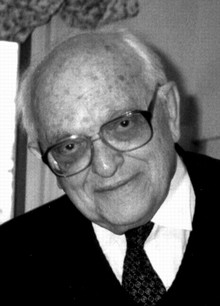
\includegraphics[scale=0.2]{MPI - Maths/Expose/images/Anatol_Rapoport.jpg}
        
            Anatol Rapoport (1911 - 2017)
        \end{center}
        
        \column{0.5\textwidth}
        \begin{center}
            \emph{à quoi ressemble un graphe \guill{typique} avec $n$ sommets et $m$ arêtes ? }\pause
            
            \begin{bform}{Idée}{}
                    Générer un graphe par un processus aléatoire \emph{(graphe aléatoire)}.
            \end{bform}
        \end{center}\pause
        
        \begin{enumerate}
            \itt Plus particulièrement, on va générer aléatoirement les arrêtes d'un graphe.
        \end{enumerate}
    \end{columns}
\end{frame}

\begin{frame}{Modèle d'Erdös et Rényi : $\bcG\p{n, p}$}
    
    Soit $n \in \bdN^*$. On considère les sommets $\iint{1, n}$. 
    
    \begin{notation}{}{}
        On note \hg{$\Omega_n$} l'ensemble des graphes \hg{$G$} tels que 
        %
        \[ \hg{V\p{G} = \iint{1, n}} \]
    \end{notation}\pause
            
    \begin{bdefinition}{Graphe complet, $K_n$}{}
        On appelle \hg{graphe complet} un graphe dont tous les sommets sont adjacents. Le graphe complet de \hg{$\Omega_n$} est noté \hg{$K_n$}.\pause
                
        \begin{columns}
            \column{0.3\textwidth}
            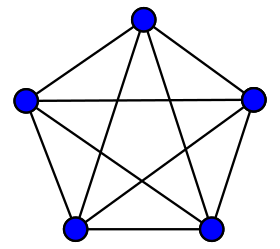
\includegraphics[scale=0.3]{MPI - Maths/Expose/images/K5.png}
                    
            \column{0.3\textwidth}
            Ci-contre $K_5$.
        \end{columns}
    \end{bdefinition}
\end{frame}

\begin{frame}{Modèle d'Erdös et Rényi : $\bcG\p{n, p}$}
    
    \begin{bdefinition}{$\bcG\p{n, p}$}{}
        Soient \hg{$n \in \bdN^*$}, \hg{$p \in \intc{0, 1}$}, et pour \hg{$e \in E\p{K_n}$}, la variable aléatoire telle que
        %
        \[ \hg{X_e \hookrightarrow \bcB\p{p}} \]
        %
        On appelle \hg{graphe aléatoire binomial} (d'\textsc{Erdös} et \textsc{Rényi}) la \hg{variable aléatoire $\bcG\p{n, p} = \p{\iint{1, n}, E_\bcG}$} dans $\Omega_n$ telle que
        %
        \[ \hg{\forall e \in E\p{K_n},\qquad \p{e \in E_\bcG} = \p{X_e = 1}}\]
    \end{bdefinition}\pause
    
    Autrement dit, on chaque arrête de $K_n$, a une probabilité $p$.\pause 
    
    On remarque (d'où le nom de binomial) :
    %
    \[ \mod{E_\bcG} \hookrightarrow \bcB\p{\dfrac{n\p{n-1}}{2}, p} = \bcB\p{\vphantom{\dfrac{n\p{n-1}}{2}}\mod{E\p{K_n}}, p}\]
\end{frame}

\begin{frame}{Modèle d'Erdös et Rényi : $\bcG\p{n, p}$}
    \begin{bexample}{}{}
        \begin{columns}
            \column{0.33\textwidth}
            \centering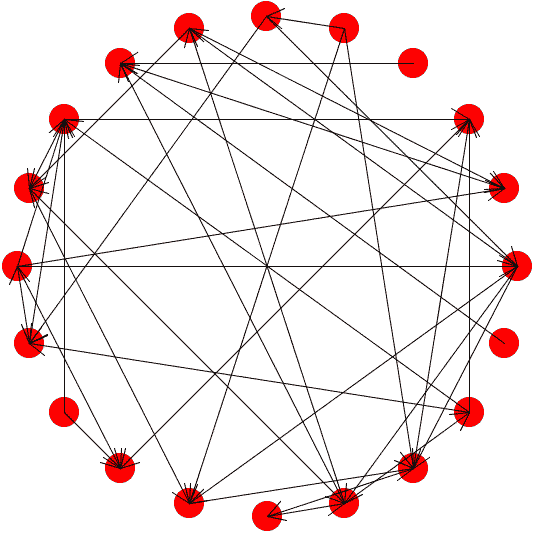
\includegraphics[scale=0.16]{MPI - Maths/Expose/images/exG1.png}
                    
            \column{0.33\textwidth}
            \centering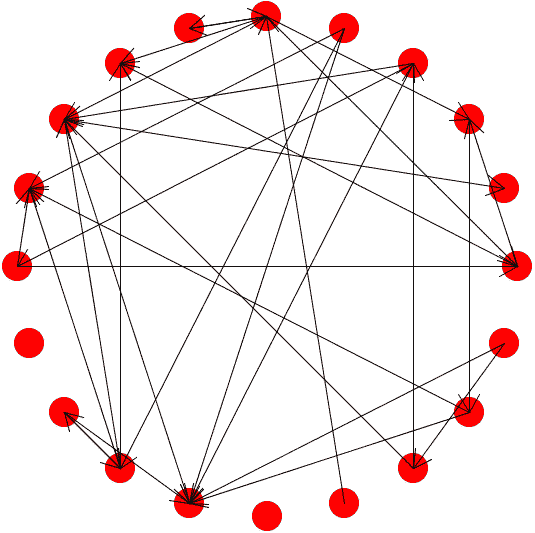
\includegraphics[scale=0.16]{MPI - Maths/Expose/images/exG2.png}
            
            \column{0.33\textwidth}
            \centering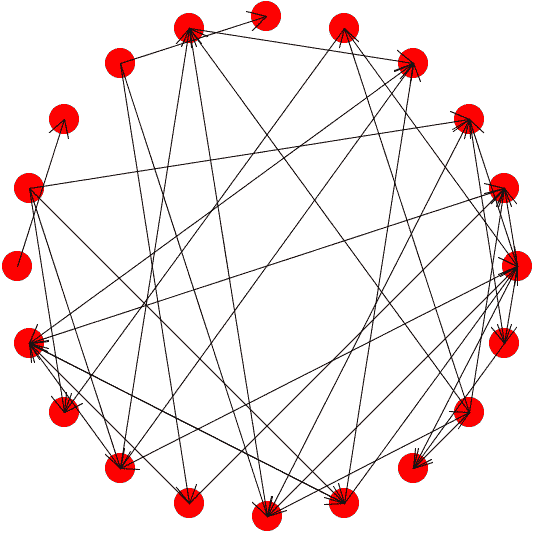
\includegraphics[scale=0.16]{MPI - Maths/Expose/images/exG3.png}
        \end{columns}
        
        \begin{center}
            $\bcG\p{n, p}$ avec $n = 20$ et $p = 0,1$.
        \end{center}
    \end{bexample}\pause
    
    Dans la suite, on considérera des propriétés asymptotiques du graphe aléatoire binomial, c'est-à-dire pour un grand nombre de sommets.\pause
    
    \centering On étudiera donc $\bcG\p{n, p}$ lorsque $n$ tend vers $+\infty$.
\end{frame}

\begin{frame}{Modèle d'Erdös et Rényi : $\bdG\p{n, M}$}
    
    \begin{bdefinition}{$\bdG\p{n, M}$}{}
        Soient \hg{$n \in \bdN^*$}, et $M$ un sous-ensemble de $E\p{K_n}$. On a
        %
        \[ \bdP\p{\bdG\p{n, M}} = \dfrac{1}{\dbinom{\frac{n\p{n-1}}{2}}{M}} \]
        %
        On parle du \hg{graphe aléatoire uniforme} (d'\textsc{Erdös} et \textsc{Rényi}).
    \end{bdefinition}\pause
\end{frame}

\begin{frame}{Petite balade chez nos amis les physiciens}
    \begin{center}
        \begin{tikzpicture}[scale=0.7]
                \coordinate (O) at (0,0.5);
                \coordinate (N1) at (5,10);
                \coordinate (N2) at (11,10);
                \coordinate (NE) at (12,10);
                \coordinate (NW) at (0,10);
                \coordinate (SE) at (12,0);
                \coordinate (SW) at (0, 0);
                \coordinate (W) at (0,5);
                \coordinate (S) at (6,0);
                \coordinate (C) at (10.2,7.8); % critical
                \coordinate (T) at (4,3); % triple
                
                % CHEMINS
                \def\SL{(T) -- (N1)}
                \def\SG{(O) to[out=20,in=-120] (T)}
                \def\LG{(T) to[out=20,in=-120] (C)}
                \def\atm{(0,5.5) -- (12,5.5)}
                \path[name path=SL] \SL;
                \path[name path=LG] \LG;
                \path[name path=atm] \atm;
                
                % REGIONS
                \fill[main7!20] \SG -- (N1) -- (NW) -- cycle;
                \fill[main1!20] \LG -- (N2) -- (N1) -- cycle;
                \fill[main4!20] \LG -- (N2) -- (NE) -- (SE) -- (SW) -- \SG -- cycle;
                
                
                %LIGNES
                \draw[thick] \SG;
                \draw[thick] \LG;
                \draw[thick] \SL;
                
                \pause
                \node at (2,5) {\color{main7} Solide (S)};
                \node at (8,2.2) {\color{main4} Vapeur / Gaz (G)};
                \node at (6.5,6.6) {\color{main1} Liquide (L)};
                
                % POINTS
                \fill[] (C) circle (1.5pt) node[above=1pt,scale=0.6,align=center] {C};
                \fill[main10] (T) circle (3pt) node[below right,main10,scale=0.9,align=right] {\textsc{iii}};
        \end{tikzpicture}
    \end{center}
\end{frame}

\begin{frame}{Petite balade chez nos amis les physiciens}
    \centering Modèle d'\textsc{Ising}
\end{frame}

\begin{frame}{Phénomènes de seuil}

    \begin{enumerate}
        \itt Il est intéressant d'étudier les propriétés de $\bcG\p{n, p}$ (formellement un sous ensemble de $\Omega_n$) au fur et à mesure que $p$ évolue : on parle de \emph{schéma d'évolution}.\pause
        
        \itt En étudiant de tels schéma, Erdős et Rényi ont découvert que ces propriétés n'évoluait pas de manière continue, et qu'il y avait un phénomène de \guill{changement de phase} : lorsque $p$ dépasse une valeur $p_\text c$, le graphe change radicalement.
    \end{enumerate}
    %
    \pause
    
    \begin{bdefinition}{Propriété vérifiée a.p.s}{}
        On dit qu'une propriété $\bcP$ sur $\bcG\p{n, p}$ est \hg{vérifie asymptotiquement presque sûrement (a.p.s)} lorsque
        %
        \[ \hg{\bbP\p{\bcG\p{n, p} \in \bcP} \lima{n \to +\infty} 1}\]
        %
        Notons que $p$ peut être une fonction de $n$.
    \end{bdefinition}
\end{frame}

\begin{frame}{Phénomènes de seuil}
    \begin{bform}{Idée}{}
            Pour des propriété $\bcP$ sur $\bcG\p{n, p}$, il existe $p_\text c\p{n} \in \intc{0, 1}$ tel que :
            %
            \[ \begin{cases}
                p \ \text{petit devant} \ p_\text c\p{n} &\implies \bcP \ \text{fausse a.p.s}\\
                p \ \text{grand devant} \ p_\text c\p{n} &\implies \bcP \ \text{vraie a.p.s}
            \end{cases}\]
            %
            \pause
            %
            On dit que $p_\text c\p{n}$ est une \emph{fonction de seuil} et que $\bcP$ vérifie un \emph{phénomène de seuil}.
    \end{bform}
\end{frame}

\begin{frame}{Phénomènes de seuil}
    \begin{bproperty}{Méthode du premier moment}{}
        Soit \hg{$\p{X_n}_{n \in \bdN^*}$} une suite de \hg{v.a. à valeurs dans $\bdN$}.
        %
        \[ \hg{\lim\limits_{n \to +\infty} \bdE\p{X_n} = 0 \implies \p{X_n = 0} \ \text{a.p.s}} \]
    \end{bproperty}
    \pause
    \begin{nproof}
        On applique l'inégalité de \textsc{Markov} :
        %
        \[ \bbP\p{X_n > 0} = \bdP\p{X_n \geq 1} \leq \dfrac{\bdE\p{X_n}}{1} \lima{n \to +\infty} 0\]
    \end{nproof}\pause
    
    Notamment, si $X_n$ compte \guill{combien de fois} un $\bcP$ est vérifié dans $\bcG\p{n, p}$, alors $\bcG\p{n,p}$ ne vérifie pas $\bcP$.
\end{frame}

\begin{frame}{Phénomènes de seuil}
    \begin{bexercise}{}{}
        Compter le nombre moyen de copies de $K_4$ dans $\bcG\p{n,p}$. Montrer que si $p = \bco\p{\dfrac{1}{n^{2/3}}}$ alors a.p.s $\bcG\p{n,p}$ ne contient pas de copie de $K_4$.
    \end{bexercise}
\end{frame}

\begin{frame}{Phénomènes de seuil}
    \begin{bproperty}{Méthode du deuxième moment}{}
        Soit \hg{$\p{X_n}_{n \in \bdN^*}$} une suite de \hg{v.a. à valeurs dans $\bdN$} non nulle.
        %
        \[ \hg{\sigma\p{X_n} = \bco\p{\bdE\p{X_n}} \implies \p{X_n > 0} \ \text{a.p.s}} \]
    \end{bproperty}
    \pause
    \begin{nproof}Par \textsc{Cauchy-Schwarz} :
        \[ \bdE\p{X_n}^2 = \bdE\p{X_nI_{X_n > 0}}^2 \leq \bdE\p{X_n^2}\bdE\p{I_{X_n > 0}^2} = \bdE\p{X_n^2}\bbP\p{X_n > 0}\]
        %
        D'où :
        %
        \[\bbP\p{X_n \geq 1} = \bbP\p{X_n > 0} \geq \dfrac{\bdE\p{X_n}^2}{\bdE\p{X_n^2}} = 1 - \dfrac{\bdV\p{X_n}}{\bdE\p{X_n^2}} \geq 1 - \p{\dfrac{\sigma\p{X_n}}{\bdE\p{X_n}}}^2\]
    \end{nproof}\pause
\end{frame}

\begin{frame}{Phénomènes de seuil}
    \begin{bexercise}{}{}
        Montrer que si $p = \bco\p{\dfrac{1}{n^2}}$, alors $\bcG\p{n,p}$ est a.p.s le graphe vide. Montrer que si $p = \dfrac{1}{\sqrt{n}}$, alors $\bcG\p{n,p}$ est a.p.s non vide.
    \end{bexercise}
\end{frame}

\begin{frame}{Propriétés croissantes}
    \begin{bdefinition}{Propriété croissante}{}
        On dit qu'une propriété \hg{$\bcP$ est croissante} lorsque
        %
        \[ \hg{\forall A \subset \bcP, \forall B \subset \Omega_n,\qquad A \subset B \implies B \subset \bcP}\]
    \end{bdefinition}\pause
    
    \begin{btheorem}{}{}
        Soient \hg{$\bcP$ une propriété croissante} non triviale ($\bcP \neq \Omega_n$ et $\bcP \neq \emptyset$). La fonction
        %
        \[ p \mapsto \bbP\p{\bcG\p{p, n} \in \bcP} \]
        %
        est croissante de $0$ à $1$ d'où \hg{$\bcP$ vérifie un phénomène de seuil}.
    \end{btheorem}
    
     
\end{frame}

\begin{frame}{Cas de $\bdZ^2$ : théorie de la percolation}
    \begin{enumerate}
        \itt On considère le graphe $2$-dimensionnel dont les sommets correspondent aux éléments de $\bdZ^2$\pause
        
        \itt Pour chaque arrête $e$ potentielle (horizontale ou verticale) entre deux sommets, on génère un nombre aléatoire $p_e \in \intc{0, 1}$.\pause
        
        \itt Pour un $p \in \int{0, 1}$ donné, on considère le graphe $G = \p{Z^2, E}$ tel que $e \in E$ si et seulement $p \geq p_e$. On a donc un graphe aléatoire binomial pour lequel on peut étudier un schéma d'évolution.\pause
        
        \itt Pour visualiser, on colore les composantes connexes d'une même couleur.
    \end{enumerate}
\end{frame}

\begin{frame}{Cas de $\bdZ^2$ : théorie de la percolation}
    
    Questions :
    %
    \begin{enumerate}
        \itt<1-> Quelle est la valeur critique $p_\text c$ ?
        
        \itb<5-> \emph{Réponse :} $p_\text c = 0,5$
        
        \itt<2-> Y-a-t-il plus d'une composante connexe infinie ?
        
        \itb<6-> \emph{Réponse :} Non
        
        \itt<3-> A quelle vitesse la transition de phase a-t-elle lieu ?
        
        \itb<7-> \emph{Réponse partielle :} \guill{asymptotique} en $n^{-3/4}$ quand $n$
        
        \itt<4-> Quelle taille ont les composantes connexes avant de \guill{fusionner} ?
        
        \itb<8-> \emph{Réponse partielles :} \guill{asymptotique} en $\p{p - p_\text c}^{-43/18}$
    \end{enumerate}
\end{frame}

\begin{frame}{Existence d'une valeur critique}
    Dans la suite, on note $\bcC_\infty$ la propriété : 
    %
    \begin{center}
        \guill{il existe une composante connexe infinie dans le graphe}.\pause
    \end{center}
    
    On cherchera à montrer le théorème suivant :
    %
    \begin{btheorem}{Rudolph Peierls (1907-1995)}{}
        Il existe \hg{$p_\text c \in \into{0, 1}$} tel que 
        %
        \[ \hg{\begin{cases}
                p < p_\text c \implies \bbP_p\p{\bcC_\infty} = 0\\
                p > p_\text c \implies \bbP_p\p{\bcC_\infty} = 1
            \end{cases}}
         \]
    \end{btheorem}
    
\end{frame}

\begin{frame}{Loi du zéro-un de Kolmogorov}
    \begin{blemma}{$\bcC_\infty$ quasi-certain ou quasi-impossible}{}
        \[ \hg{\bbP_p\p{\bcC_\infty} = \ens{0, 1}}\]
    \end{blemma}
    
    \begin{nproof}
        Supposons que $\bbP_p\p{\bcC_\infty} \neq 0$. On note $\bfR$ l'ensemble des états de sous-ensembles fini d'arêtes du graphe, $\bcT$ la tribu engendrée par $\bfR$.\pause
        %
        \[ \forall A \in \bfR,\qquad \bbP_p\p{\bcC_\infty \enstq A} = \bbP_p\p{\bcC_\infty}\]
        %
        \pause Dès lors par \textsc{Bayes}, on a $\bbP_p\p{A} = \bbP_p\p{A \enstq \bcC_\infty}$ pour $A \in \bcT$.\pause
        
        Or $\bcC_\infty \in \bcT$ d'où $\bbP_p\p{\bcC_\infty} = \bbP_p\p{\bcC_\infty \enstq \bcC_\infty} = 1$.
    \end{nproof}
\end{frame}

\begin{frame}{Invariance d'origine}
    
    Pour $O \in \bdZ^2$, on note $\bcC_{\infty, O}$ la propriété : 
    %
    \begin{center}
        \guill{la composante connexe en $O$ est infinie}
    \end{center}\pause
    
    \begin{blemma}{$\bbP_p\p{\bcC_{\infty, O}}$}{}
        \[ \hg{\begin{cases}
                \bbP_p\p{\bcC_{\infty, O}} = 0 \iff \bbP_p\p{\bcC_{\infty}} = 0\\
                \bbP_p\p{\bcC_{\infty, O}} > 0 \iff \bbP_p\p{\bcC_{\infty}} = 1
            \end{cases}}\]
    \end{blemma}\pause
    
    \begin{nproof}
        On a $\bbP_p\p{\bcC_{\infty, O}} \leq \bbP_p\p{\bcC_{\infty}}$ donc
        %
        %
        \[ \begin{cases}
            \bbP_p\p{\bcC_{\infty}} = 0 &\implies \bbP_p\p{\bcC_{\infty, O}} = 0\\ \bbP_p\p{\bcC_{\infty, O}} > 0 &\implies \bbP_p\p{\bcC_{\infty}} = 1
            \end{cases} \]
        %
        On termine par contraposée.
    \end{nproof}
    
\end{frame}

\begin{frame}{Existence de $p_\text c \in \intc{0, 1}$}
    
    On remarque (admet) que $\bcC_{\infty, O}$ est croissante, \ie
    %
    \[ \forall \p{p_1, p_2} \in \intc{0, 1}^2,\qquad p_1 \leq p_2 \implies \bbP_{p_1}\p{\bcC_{\infty, O}} \leq \bbP_{p_2}\p{\bcC_{\infty, O}}\]
    %
    \pause
    %
    Par ailleurs il est clair que $\bbP_0\p{\bcC_{\infty, O}} = 0$ et $\bbP_1\p{\bcC_{\infty, O}} = 1$, on peut donc poser
    %
    \[ p_\text c = \sup \ens{p \in \intc{0, 1} \enstq \bbP_p\p{\bcC_{\infty, O}} = 0}\]
    %
    \pause On a donc
    %
    \[ \begin{cases}
            p < p_\text c \implies \bbP_p\p{\bcC_\infty} = 0\\
            p > p_\text c \implies \bbP_p\p{\bcC_\infty} = 1
        \end{cases}
    \]
    %
    \pause Il reste alors à montrer que $p_\text c \not\in \ens{0, 1}$.
    
\end{frame}

\begin{frame}{$p_\text c > 0$}

    Pour $\ell \in \bdN^*$, on note $\bcC_{\ell, O}$ la propriété : 
    %
    \begin{center}
        \guill{il existe un chemin de longueur $\ell$ partant de $O$}
    \end{center}\pause
    
    \begin{blemma}{$p_c \neq 0$}{}
        \[ \hg{p_\text c \geq 1/3}\]
    \end{blemma}\pause
    
    \begin{nproof}
        On a $\bbP_p\p{\bcC_{\infty, O}} \leq \bbP_p\p{\bcC_{\infty, \ell}}\pause \leq \displaystyle \sum_{\Gamma \ \text{de longueur \ell}} p^\ell$.\pause
        
        Or $\displaystyle \sum_{\Gamma \ \text{de longueur \ell}} p^\ell \leq p^\ell \mod{\ens{\Gamma \ \text{de longueur \ell}}}$.\pause
        
        De plus $\mod{\ens{\Gamma \ \text{de longueur \ell}}} \leq 4\cdot 3^{\ell - 1}$. D'où
        %
        \[ p < \dfrac{1}{3} \implies \bbP_p\p{\bcC_{\infty, O}} \leq 4p\p{3p}^{\ell - 1} \lima{\ell \to +\infty} 0\]
        %
        Donc $p_\text c \geq 0$.
    \end{nproof}
\end{frame}

\begin{frame}{$p_\text c < 1$}
    \begin{blemma}{$p_\text c \neq 1$}{}
        \[ \hg{p_\text c \leq 2/3 }\]
    \end{blemma}
\end{frame}

\begin{frame}{Conclusion}
        \begin{btheorem}{Rudolph Peierls (1907-1995)}{}
        Il existe \hg{$p_\text c \in \intc{\dfrac{1}{3}, \dfrac{2}{3}}$} tel que 
        %
        \[ \hg{\begin{cases}
                p < p_\text c \implies \bbP_p\p{\bcC_\infty} = 0\\
                p > p_\text c \implies \bbP_p\p{\bcC_\infty} = 1
            \end{cases}}
         \]
    \end{btheorem}
\end{frame}






\end{document}